\documentclass[12pt]{article}
\usepackage{amssymb}
\usepackage{amsmath}
\usepackage{tikz}
\usepackage{graphicx}
\usepackage{subfig}
\usepackage[font=footnotesize,labelfont=bf]{caption}
\usepackage[export]{adjustbox}
\graphicspath{ {./Code/figures} }
\usetikzlibrary{fit}
\renewcommand{\baselinestretch}{1.2}
\newcommand{\partialderiv}[2]{\frac{\partial #1}{\partial #2}}

\begin{document}
\begin{center}
\Large
Attention-Based Learning Rule Provides Biological Basis for Backpropagation in the Human Brain
\end{center}

\begin{center}
Avi Balsam \\
Hebrew University of Jerusalem\\
\verb+avi.balsam@mail.huji.ac.il+\\
\vspace{0.2cm}
Dr. Oren Forkosh\\
Hebrew University of Jerusalem\\
\verb+oren.forkosh@mail.huji.ac.il+
\end{center}

%TODO: Add methods section for technical stuff, make brief paragraph which summarizes the backpropagation algo in a less rigorous way (just 3 neurons). Done.
%TODO: Our method doesn't count as retrograde signaling. Fixed.
\section{Abstract}
Backpropagation, the algorithm fundamental to the operation of artificial neural networks, has yet to be observed in the human brain. In particular, while backpropagation relies on an error signal transmitted through the network in a retrograde manner, study of human neural networks generally treats neurons as independent units which do not coordinate on a global level to optimize their weights. While the potential for retrograde signaling exists in neurons, it is not clear whether these signals propagate over long distances, let alone throughout the entire network. In this paper, we show that a learning rule equivalent to backpropagation can be developed from a local optimization paradigm in which neurons only communicate with their immediate neighbors and seek to optimize a local cost function. We outline one possible learning rule with this property and show that it is mathematically equivalent to the classical backpropagation algorithm developed by Rumelhart et. al. We then solve a fundamental problem with our model's biological plausibility using attention mechanisms. Using our modified algorithm, we were able to train a neural network on a simple task, and we believe our algorithm is capable of learning more complicated functions. Our research establishes one more link between artificial and human neural networks, fostering a more complete understanding of both.

\section{Introduction}
Synaptic plasticity has long been recognized as an important factor in neural learning. James \cite{James1890} proposed that ``the phenomena of habit in living beings are due to the plasticity of the organic materials of which their bodies are composed.'' Later, Hebb \cite{Hebb1949} theorized that the connection between a pre- and postsynaptic neuron would be strengthened if the presynaptic neuron fired before the postsynaptic neuron, and weakened if the reverse was the case. This model has been refined over the years. \cite{Markram2012} Its more modern descendant, dubbed spike-time-dependent plasticity or STDP, includes both Hebbian and ``anti-Hebbian'' learning rules which are essentially the inverse of Hebb's model. \cite{Carlson1990} Many of the mechanisms underlying STDP have been observed in human and animal brains. \cite{Markram2011} However, the concept still requires more explanation on a theoretical level, to determine the computational mechanisms that are a consequence of STDP. In other words, while it seems clear that STDP is a feature of connections between neurons, further study is required to outline the computational and representational purpose of modulated changes in the strength of synaptic connections.

To explain the nature of neuronal representations of memory and stimuli, Hebb theorized that neurons act in groups, or ``assemblies,'' each of which represents some ``distinct cognitive entity.'' \cite{Hebb1949} Further work has established that there is a hierarchical structure to these assemblies in which ``downstream `observer-reader-classifier-integrator' mechanisms'' synthesize data from other neurons representing lower-level features of stimulus data. \cite{Buzsaki2010} This framework brings to mind artificial neural networks, since they also exhibit a hierarchy in which deeper layers store higher-level features. \cite{HighLevelFeaturesANN} However, while artificial neural networks use backpropagation to allow for efficient learning even in networks with many parameters, \cite{backprop} neural networks in the brain do not coordinate on a global level to optimize their weights (synaptic efficiencies) and biases (excitabilities). \cite{Dahmen2022} Instead, when developing theoretical models to understand the computational power of STDP, our learning rules must operate on the level of the individual neuron. Somehow, neurons' local optimizations must lead to global learning behaviors. In this paper, we develop a learning rule with this property, and show that it is, in fact, equivalent to backpropagation.

Studies have shown that an agent must focus its attention on an object for a relatively long period of time in order to learn. \cite{Desimone2014} We theorize that attention can solve the two-phase problem, a fundamental issue we will pose regarding the biological plausibility of our learning rule. In particular, attention to an object decreases temporal differentiation in neuronal activations, allowing both steps of the backpropagation algorithm to occur synchronously.

\subsection{Retrograde Signaling in the Brain}
Although synapses were for years considered ``one way streets,'' it is now known that there are signaling molecules capable of crossing the synaptic cleft in a retrograde manner. \cite{Tao2001} These molecules include proteins such as neurotrophins, \cite{Dechant2003} gases, \cite{RodriguezGrande2017} and lipids such as endocannaboids. \cite{Mechoulam1998} It is widely theorized that the retrosynaptic transmission of these molecules plays a role in synaptic plasticity. \cite{EAlger2002} \cite{Schuman1999} We review some proposed mechanisms for retrograde signaling in the brain.

\subsubsection{Neurotrophins}
Neurotrophins (NTs) are a family of proteins which are vital for the proper development of the vertebrate nervous system. \cite{Tao2001} NTs can change synaptic efficacy by affecting both the frequency and amplitude of synaptic currents. \cite{Levine1995} Along with the fact that expression levels of NTs are sensitive to electrical activity, this suggests that NTs are a factor in synaptic plasticity. Moreover, the fact that NTs are known to be transported in a retroaxonal manner \cite{Hendry1974} suggests that may be involved in the retrograde propagation of synaptic plasticity.

\subsubsection{Endocannabinoids}
The brain cannabinoid receptor (CB1) is expressed in high levels in the cortex, hippocampus, cerebellum and basal ganglia. \cite{Wilson2002} So far, two lipids have been identified as CB1 agonists. Unlike most neurotransmitters, these agonists are not stored, but rather rapidly synthesized in response to depolarization. Experiments (\cite{Pitler1992}, \cite{Llano1991}) have shown that brief depolarization of a neuron can suppress inhibitory GABAergic synaptic events in that cell. This phenomena is known as ``depolarization‐induced suppression of inhibition'' or DSI. It was shown that DSI affects the presynaptic terminal even though it originates from the postsynaptic neuron. Endocannabinoid signals are essentially very local and do not diffuse widely to vast brain areas. \cite{Wilson2001} While Fitzsimonds et al. \cite{Fitzsimons1997} have noted that such a retrograde signal naturally evokes the backpropagation algorithm, the computational role of these retrograde signals has not been studied in depth.

\subsection{Limitations of Retrograde Signaling}
Although it is possible that the brain backpropagates using these retrograde signals, there is good reason to study the theory that the plasticity is primarily driven by the firing of action potentials, or the anteretrograde transmission of neurotransmitters across the synaptic cleft. Besides for their simplicitly, action-potential-driven theories of cognition are backed by numerous studies which highlight the seemingly extraneous role retrograde processes such as the transmission of NTs and endocannaboids play in synaptic plasticity. The retrograde signal propagated by NTs takes minutes to propagate along the axon, \cite{Poo2001} in contrast to action potentials, which propagate across synapses in milliseconds. Endocannabinoid-based retrograde signals are not well-understood. \cite{OhnoShosaku2014} Additionally, it is not known whether the aforementioned retrograde signals propagate over large distances. \cite{Matusica2014}

As such, we would like a local learning rule in which neurons only use information immediately available to them to compute the change in their weights and biases, without relying on long-distance retrograde signaling. The learning rule that we will develop has this property, and it therefore allows for backpropagation even without a long-distance retrograde transfer of information.

\subsection{Neural Networks}
To model interactions in the brain, we will use a simple feedforward neural network. While in reality neurons fire action potential spikes to transmit information, we can model the behavior of spiking neurons by using their firing rate, or the number of spikes per unit of time, as their activation. We lose information with this model, since the temporal positioning of the spikes may encode information. By modelling the brain with an artificial neural network, we assume that the brain encodes information in the firing rates of neurons without taking into account the exact times of action potential spikes.

A neural network is a list of layers of neurons. Each neuron in a layer has a weighted connection to all neurons in the next layer. When processing an input, defined as a vector $a_{\text{inp}}$, the network sets the activations of its first layer, $a^0$, equal to $a_{\text{inp}}$. To calculate the activation of a neuron in a subsequent layer, the network multiplies the weights of each incoming synapse (connection) by the activation of the presynaptic neuron, then adds them together. Next, the neuron adds its bias, a parameter which is also learned, and inputs the result to a nonlinear activation function $\sigma$. To make future calculations easier, we will the bias of a neuron with bias $b$ as a separate neuron with an activation of one and a weight of $b$.

\begin{figure}
	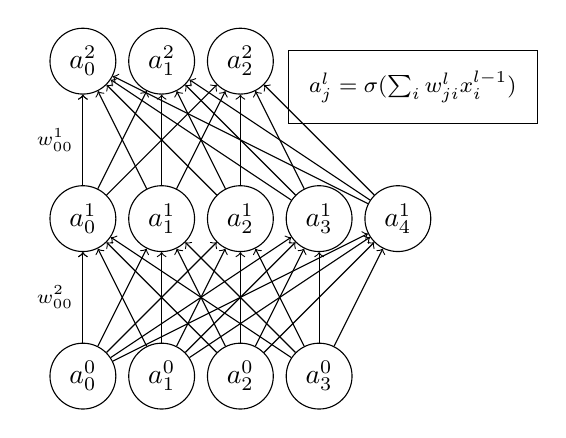
\begin{tikzpicture}[
		node distance=1.8cm,
		input/.style={circle, draw, minimum size=0.8cm},
		weight/.style={midway, left, font=\scriptsize, fill=white}
		]
		
		% Activation formula (general)
		\node[align=left, anchor=north west, font=\footnotesize] at (3.75, 4) (formula) {$a_j^l = \sigma(\sum_i w_{ji}^l x_i^{l-1})$};
		\node[draw=black, inner sep=4pt, fit=(formula)] (border) {};
		
		% Input layer nodes
		\foreach \i/\label in {1/$a_0^0$, 2/$a_1^0$, 3/$a_2^0$, 4/$a_3^0$}
		\node[input] (input\i) at (\i,0) {\label};
		
		% Hidden layer nodes
		\foreach \i/\label in {1/$a_0^1$, 2/$a_1^1$, 3/$a_2^1$, 4/$a_3^1$, 5/$a_4^1$}
		\node[input] (hidden\i) at (\i,2) {\label};
		
		% Output layer nodes
		\foreach \i/\label in {1/$a_0^2$, 2/$a_1^2$, 3/$a_2^2$}
		\node[input] (output\i) at (\i,4) {\label};
		
		% Arrows between layers and weight labels
		\foreach \i in {1, ..., 4}
		\foreach \j in {1, ..., 5}
		{
			\draw[->] (input\i) -- (hidden\j);
		}
		
		\foreach \i in {1, ..., 5}
		\foreach \j in {1, ..., 3}
		{
			\draw[->] (hidden\i) -- (output\j);
		}
		
		% One weight label for each layer
		\draw[->] (input1) -- (hidden1) node[weight] {$w^{2}_{00}$};
		\draw[->] (hidden1) -- (output1) node[weight] {$w^{1}_{00}$};
		
	\end{tikzpicture}\centering
	\caption{Diagram of a neural network. Arrows represent weights, and nodes represent neurons, each with its own activation. The notation used here is the notation used throughout the paper. Note: When indexing the weight matrix, the first index is the index of the postsynaptic neuron, and the second is the index of the presynaptic neuron. Hence, $w^l_{jk}$ refers to the weight of the connection from the $k$-th neuron in the $(l-1)$-th layer to the $j$-th neuron in the $l$-th layer.}
\end{figure}

Neural networks attempt to optimize their weights to fit some target function $X$ by calculating the gradient of $X$ with respect to the weights of the network. This computation can be efficiently performed using backpropagation, the mathematics of which will be detailed in the ``Methods'' section. Once the gradient has been calculated, neurons modify their weights in the direction of steepest descent, namely the negation of the gradient.

\subsection{Synaptic Echo}
After a neuron releases an action potential spike, excess neurotransmitter not accepted by the postsynaptic neuron is reabsorbed into the presynaptic neuron by way of various transport mechanisms. \cite{Rudnick1993} This reuptake allows the presynaptic neuron to recycle neurotransmitter, thereby increasing its stores of releasable molecules. \cite{Rudnick1993} Many studies have explored the role of reuptake mechanisms and transporters in modulating synaptic plasticity. \cite{Duman2016} In fact, drugs such as amphetamines and opiates specifically target neurotransmitter receptors, thereby increasing extracellular neurotransmitter concentration and modulating synaptic plasticity. \cite{Amara1998}

While much of the research on synaptic reuptake has focused on the ability of extracellular neurotransmitter to alter reward pathways in the brain, \cite{Koob1992} we believe that reuptake may play a fundamental role in neural learning. Specifically, the quantity of neurotransmitter reabsorbed by presynaptic receptors is a function of the neuron's activation and the efficacy of the synapse. Using the ``synaptic echo'' reuptake provides, a presynaptic neuron can estimate, with a significant degree of accuracy, the synaptic efficacy of its connection to a postsynaptic neuron. This will prove important when deriving our learning rule, as neurons will use changes in the strengths of their outgoing connections to modulate changes in incoming connections.

\section{Results}
\subsection{Simplified Derivation}
In order to simplify the derivation of our local learning rule, we will derive it for a neural network with only three layers, each containing a single neuron. We start by deriving the backpropagation algorithm for this network, and then manipulate the algorithm to make it biologically plausible. A more rigorous overview of backpropagation and our learning rule with more mathematical context can be found in the ``Methods'' section. Here, we will denote the activations of the neurons as $a_0$, $a_1$, and $a_2$, the weights as $w_1$ and $w_2$, the biases as $b_1$ and $b_2$, and the network's activation function (which we assume is the same for all neurons) as $\sigma$. An illustration of the network can be found in figure \ref{fig:simple_ann_diagram}.

\begin{figure}
	\begin{center}
	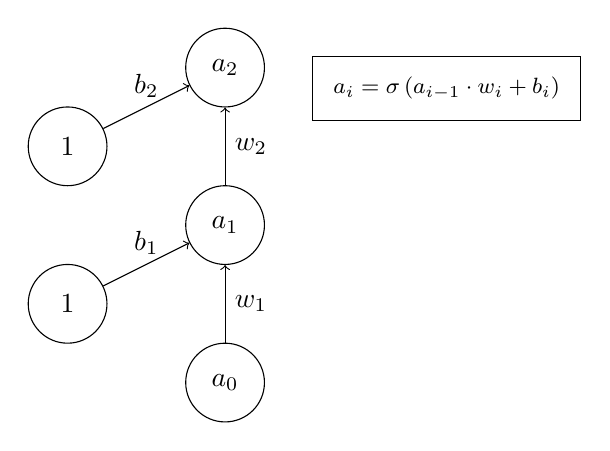
\begin{tikzpicture}[scale=1.0]
		% Activation formula
		\node[align=left, anchor=north west, font=\footnotesize] at (1.25, 4) (formula) {$a_i = \sigma\left(a_{i-1}\cdot w_i+b_i\right)$};
		\node[draw=black, inner sep=4pt, fit=(formula)] (border) {};
		
		% Input layer
		\node[circle, draw=black, minimum size=1cm] (input) at (0,0) {$a_0$};
		
		% Hidden layer
		\node[circle, draw=black, minimum size=1cm] (hidden) at (0,2) {$a_1$};
		\node[circle, draw=black, minimum size=1cm] (hidden_prev) at (-2,1) {1};
		
		% Output layer
		\node[circle, draw=black, minimum size=1cm] (output) at (0,4) {$a_2$};
		\node[circle, draw=black, minimum size=1cm] (output_prev) at (-2,3) {1};
		
		% Connect layers
		\draw[->] (input) -- node[midway, right] {$w_1$} (hidden);
		\draw[->] (hidden_prev) -- node[midway, left, above] {$b_1$} (hidden);
		\draw[->] (hidden) -- node[midway, right] {$w_2$} (output);
		\draw[->] (output_prev) -- node[midway, left, above] {$b_2$} (output);
	\end{tikzpicture}
	\caption{Diagram of a simple neural network used to simplify derivation of our local learning rule.}\label{fig:simple_ann_diagram}
	\end{center}
\end{figure}

First, we define $z_i \equiv w_ia_{i-1} + b_i$. This quantity represents the weighted input to neuron $i$, and will be useful to make the notation simpler. Now, we define an ``error'' $\delta_i$ for each neuron, which represents the extent to which the input to that neuron contributes to undesired changes in the cost function $C$, or the partial derivative of the cost function in terms of the weighted input to that neuron $\partialderiv{C}{z_i}$. For the output neuron, we can directly compute the partial derivative of the cost function in terms of its activation $a_2$. However, this does not give us the partial derivative in terms of the \emph{input} to the neuron $z_2$, because of the nonlinearity $\sigma$. We can compute the partial derivative using the chain rule, yielding
\begin{equation}
	\delta_2 = \partialderiv{C}{z_2} = \partialderiv{C}{a_2}\partialderiv{a_2}{z_2} = \partialderiv{C}{a_2}\cdot\sigma'\left(z_2\right)
\end{equation}
To compute $\delta_i$ for $i < 2$ given $\delta_{i+1}$, we can again use the chain rule:
\begin{equation}
	\delta_i = \partialderiv{C}{z_i} = \partialderiv{C}{z_{i+1}}\partialderiv{z_{i+1}}{z_i} = \delta_{i+1}\partialderiv{z_{i+1}}{z_i}\label{simp2}
\end{equation}
Computing this partial derivative is trivial, since
\begin{equation}
	z_{i+1} = w_{i+1}a_i + b_{i+1} = w_{i+1}\cdot\sigma(z_i)+b_{i+1}
\end{equation}
Thus,
\begin{equation}
	\partialderiv{z_{i+1}}{z_i} = w_{i+1}\cdot\sigma'(z_i)\label{simp4}
\end{equation}
Putting equations \ref{simp2} and \ref{simp4} together,
\begin{equation}
	\delta_i  = w_{i+1}\delta_{i+1}\cdot\sigma'(z_i)\label{simp5}
\end{equation}
Using the chain rule, we can derive that, for all weights $w_i$ and biases $b_i$,
\begin{equation}
	\partialderiv{C}{w_i} = \partialderiv{C}{b_i}a_{i-1} = \delta_ia_{i-1}\label{simp6}
\end{equation}
Backpropagation gives us an easy way to compute the gradient of the cost function, as we can compute $\delta_i$ for all $i$ and then find the partial derivative in terms of each $w_i$ and $b_i$. For ease of notation, we will denote $\partialderiv{C}{w_i}$ as $\Delta w_i$. Then, substituting equation \ref{simp6} into equation \ref{simp5}, we can derive a learning rule which relates $\Delta w_i$ to $\Delta w_{i+1}$:
\begin{equation}
	\Delta w_i = w_{i+1}a_{i-1}\frac{\Delta w_{i+1}}{a_i}\cdot\sigma'(z_i)
\end{equation}
Now, using the fact that $x\Delta x\approx\frac{1}{2}\Delta (x^2)$,
\begin{equation}
	\Delta w_i\approx \frac{1}{2}a_{i-1}\frac{\sigma'\left(z_i\right)}{\sigma\left(z_i\right)}\Delta \left(\left(w_{i+1}\right)^2\right)\label{simp19}
\end{equation}
This is our local learning rule, and it only uses information directly available to each individual neuron. Thus, we have created a biologically plausible learning rule equivalent to backpropagation. While we derived our rule from the backpropagation equations, it can also be derived using local optimizations on the neuronal level. In particular, if each neuron attempts to increase the weight of its outgoing connections by changing the weights of its incoming connections, we will end up with an equivalent learning rule, the derivation of which can be found in ``Methods.''

\subsection{Two-Phase Problem}
Unfortunately, there are some seemingly intractable issues which must be solved in order to establish the possibility that the human brain backpropagates. First and foremost among these is the problem of timescale. While the propagation of action potential spikes is extremely fast, neural plasticity is slow to change, on the timescale of minutes to hours for long-term changes. \cite{Wei2021} Further, the speed of transmission of the synaptic echo may be slower than the propagation of an action potential, causing further delay between activation and weight-change. Let us express this problem formally.

For the remainder of this section, let $a_j^l(t)$ be the activation of neuron $j$ at layer $l$ during discrete timestep $t$, such that $a^0(t)$ is the input to the network at time $t$. Similarly, let $\delta^l_j(t) = \partialderiv{C}{z_j^l(t)}$. We can assume that the activations effectively propagate through the network instantly. That is, all activations at a given time $a^l(t)$ can be instantly calculated from $a^0(t)$. In contrast, a neuron at layer $l$ only obtains information about $\Delta w^{l+1}(t)$ at time $t + \tau$, where $\tau$ is an arbitrary constant that is unknown to the neuron.

In classical backpropagation, the network calculates all errors $\delta^l(t)$ before accepting the next input $a^0(t+1)$. This bottleneck is necessary because the network must use the activations $a^l(t)$ to compute $\Delta w^l(t)$ with
\begin{equation}
	\Delta w_{jk}^l(t) = \delta^l_j(t)a_k^{l-1}(t).
\end{equation}

In the human brain, this strategy is simply impossible, as input stimuli must be continually processed. However, if a neuron changes its activation to $a^l_k(t+1)$ before using $a^l_k(t)$ to calculate $\Delta w_{jk}^{l+1}(t)$, it must find some way of recovering $a^l_k(t)$ or develop a strategy which renders knowledge of the activation unnecessary.

\subsection{Attention}
In order to learn, the brain must focus its attention on a given object for a relatively long period of time. \cite{Desimone2014} We theorize that this attention can be used to solve the two-phase problem. Specifically, if temporal differentiation in the inputs to a neural network is low (i.e. the brain focuses on a given object for a relatively long period of time), our modified backpropagation algorithm can function even if neurons cannot create an accurate correspondence between activation and weight-change signals. In other words, if $a(t)\approx a(t+\tau)$, where $\tau$ is the time delay of the error signal, it does not matter that we are unable to recover $a(t)$, as we can use $a(t+\tau)$ instead for an approximately correct answer.

We would like to quantify the extent to which attention can solve the two-phase problem. To do this, we simulated a simple experiment in which a mouse randomly walks across a 3x3 chessboard, and attempts to predict the color of the square it is on. For a 2x2 chessboard, this would be equivalent to a binary XOR; we chose to use a 3x3 board in order to add complexity to the problem.

\begin{figure}
	
\includegraphics[scale=0.4]{mouse_chessboard}\centering
	\caption{Visualization of an example random walk}
\end{figure}

One important factor we must take into account is the fact that, in a correctly functioning neural network, the error converges to zero. In other words, as the network trains and learns to approximate the target function, temporal variation in the error naturally decreases, and $\delta(t+\tau)$ becomes closer to $\delta(t)$ for small $\tau$. However, when the network has just begun to train and the error is large, we must decrease the speed of our random walk, thereby lowering temporal differentiation in the activation signal. To quantify this, we will divide the speed of the random walk by the norm of the output error vector $\delta^l$. If $v_0$ is the base velocity of the mouse, a hyperparameter we will set, we get the actual speed of the random walk $v$ using
\begin{equation}
	v = \frac{v_0}{\log(1+|\delta^L|)}
\end{equation}

To generate training data, we picked movements out from a two-dimensional gaussian distribution with mean zero and standard devation one, with both coordinates multiplied by $v$. At each timestep, we executed one of these movements, and used the resulting coordinates as input to the network. In other words, at each timestep the mouse moves in a random direction with normally distributed velocity that depends on the current error, and it attempts to predict the color of its current location on the chessboard.

Because computing the norm of the error for every output would take excessive computational resources, we updated the value of $|\delta^L|$ every 1000 batches. Our neural network had two input neurons, each representing a coordinate value in the range [0, 1], three hidden layers, each with 20 neurons, and a single output neuron representing the color of the input location. We used a batch size of 10, set both the learning rate and the base velocity at 0.1, and used a sigmoidal activation function. When there was no time delay between activation and error, the network was easily able to learn the target pattern, as expected. Figure \ref{fig:example} shows the error history of the network, as well as the final chessboard pattern the network learned.

\begin{figure}%
	\centering
	\subfloat[\centering Final representation]{{
\includegraphics[width=4.5cm]{final_representation_chessboard_no_attention} }}%
	\qquad
	\subfloat[\centering Error history]{{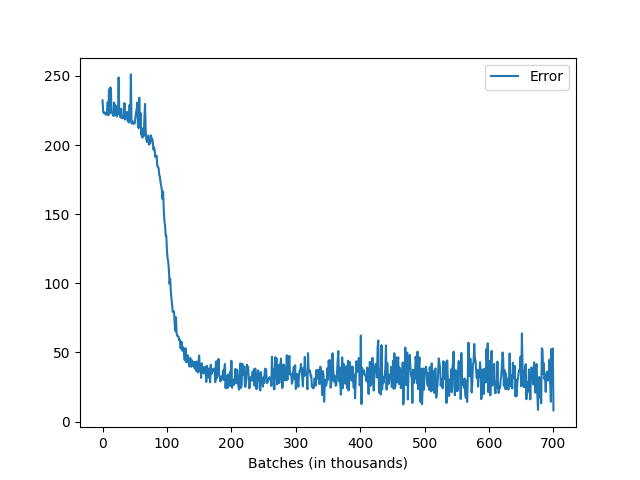
\includegraphics[width=7.5cm]{error_history_chessboard_no_attention} }}%
	\caption{Network without time delay}%
	\label{fig:example}%
\end{figure}

Next, we added a time delay between the activation and error signal. In particular, we defined a hyperparameter $\tau$, and used $\delta(t+\tau)$ in our backpropagation calculations for $a(t)$. When the inputs were not temporally correlated, the network failed to converge, as expected. In contrast, when we trained the network using our random walk simulation, it was able to successfully learn the chessboard pattern even when $\tau$ was larger than the batch size. Figure \ref{fig:various_time_delays} shows the final representations of the network at various $\tau$.

\begin{figure}%
	
	\begin{tabular}{llll}
		$\tau=5,10,15$ & 
\includegraphics[width=.2\linewidth,valign=m]{final_rep_tau_5} & 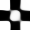
\includegraphics[width=.2\linewidth,valign=m]{final_rep_tau_10} & 
\includegraphics[width=.2\linewidth,valign=m]{final_rep_tau_15}\\
		\vspace{0.1cm}\\
		$\tau=20,25,28$ & 
\includegraphics[width=.2\linewidth,valign=m]{final_rep_tau_20} & 
\includegraphics[width=.2\linewidth,valign=m]{final_rep_tau_25} & 
\includegraphics[width=.2\linewidth,valign=m]{final_rep_tau_28}\\
	\end{tabular}
	\caption{Final representation of chessboard with various time delays.}\centering%
	\label{fig:various_time_delays}%
\end{figure}

We had hypothesized that the network would take longer to converge for larger $\tau$, and that the accuracy of the model would be inversely proportional to the value of $\tau$. Surprisingly, though, this was not the case. Figure \ref{fig:tau_convergence_speed} shows the error history of the network for different $\tau$, and figure \ref{fig:tau_final_performance} shows the final performance of the network. While for larger $\tau$ the network failed to converge completely, for $\tau\leq 20$ there does not appear to be a correlation between smaller $\tau$ and better network performance. It would seem that attention makes the network extremely robust to time delays, such that, within limits, changes in $\tau$ do not markedly impact the network's performance.

\begin{figure}
	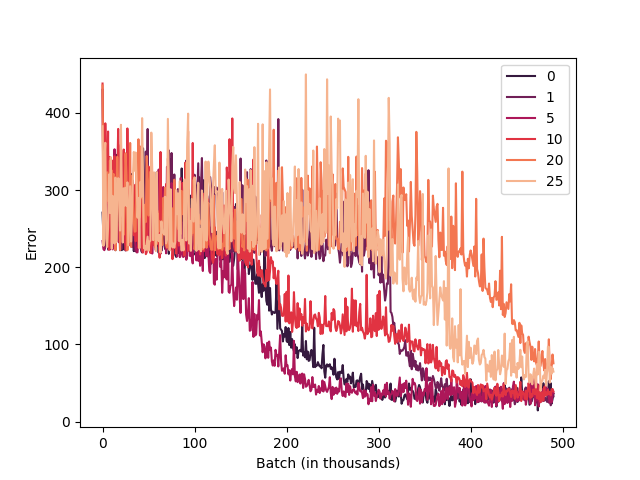
\includegraphics[width=10cm]{error_by_tau_figure}
	\centering
	\caption{Convergence of error by time delay. Each line represents a different $\tau$.}
	\label{fig:tau_convergence_speed}
\end{figure}

\begin{figure}
	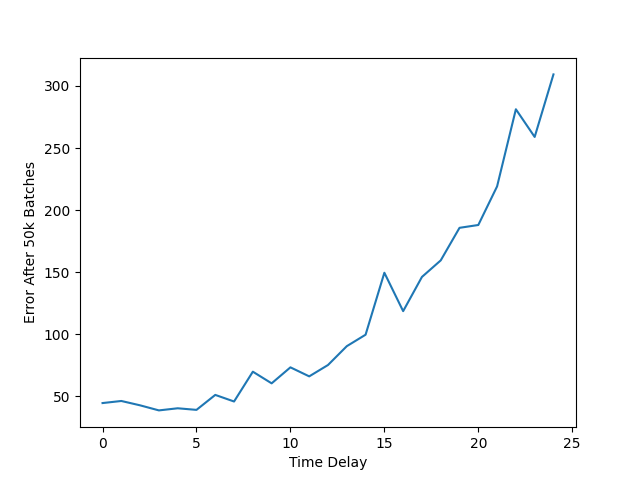
\includegraphics[width=10cm]{final_performance_by_tau}\centering
	\caption{Final performance of network by time delay.}
	\label{fig:tau_final_performance}
\end{figure}

\section{Methods}
\subsection{Backpropagation}
The following is a more rigorous overview of backpropagation, which we will use for the more general derivation of our local learning rule.

We will represent neural networks as a list of weight matrices $w^l$ such that $w^{l}_{jk}$ is the weight of the connection from the $k$-th neuron at layer $l-1$ to the $j$-th neuron at layer $l$, a list of bias vectors $b^l$ indexed by layer, and activation vectors $a^l$ such that $a^{l+1}=\sigma\left(w^{l+1}a^l + b^l\right)$, where $\sigma$ is a nonlinearity and $a^0$ is the input vector. We are given some cost function $C$ which, given an output vector $a^L$, where $L$ is the last layer of the network, returns some representation of the difference between the expected answer $y$ and $a^L$. One commonly used function is quadratic loss, where $C\left(a^L\right) = \sum_j \left(a^L_j - y_j\right)^2$.

We would like to compute the gradient of the cost function, and use that information to modify the weights and biases, thereby moving towards a minimum. In other words, we want to find $\partialderiv{C}{w^l_{jk}}$ for every weight and $\partialderiv{C}{b^l_j}$ for every bias. Once we have these quantities, we can subtract $\eta\partialderiv{C}{w^l_{jk}}$ from each $w^l_{jk}$ and $\eta\partialderiv{C}{b^l_{j}}$ from each $b^l_j$, where $\eta$ is the learning rate of the network. Repeating this process many times, we will eventually reach a minimum cost when the gradients begin to converge.

For ease of notation, we define $z_j^l \equiv w^l a^{l-1} + b^l$, so that $a^l = \sigma(z^l)$. We then define $\delta_j^l \equiv\partialderiv{C}{z_j^l}$. With a simple application of the chain rule, we can show that $\partialderiv{C}{b_j^l} = \delta_j^l$ and that $\partialderiv{C}{w_{jk}^l} = \delta_j^l a_k^{l-1}$. Therefore, computing $\delta^l$ for all $l$ is sufficient to compute the gradient of the cost function. Calculating $\delta^L$ for output layer $L$ is trivial, since the output neurons have a direct effect on the cost function:
\begin{equation}
	\delta_j^L = \partialderiv{C}{a_j^l}\cdot\sigma'\left(z_j^l\right)\label{eq1}
\end{equation}

Further, given $\delta^l$, we can compute $\delta^{l-1}$ using the following equation, which is also an application of the multivariable chain rule:
\begin{equation}
	\delta^l = \left(w^{l+1}\right)^T\delta^{l+1}\odot\sigma'\left(z^l\right)\label{eq2}
\end{equation}

After computing $\delta^l$ for all $l$ using equations \ref{eq1} and \ref{eq2}, we can compute the gradient of the cost function using the methods described above. Repeated applications of this technique will allow the network to approximate the target function.

As shown above, for the $j$-th weight at layer $l$ in a backpropagating ANN with learning rate $\eta$, backpropagation gives
\begin{equation}
	\Delta w_{jk}^l = \eta\partialderiv{C}{w_{jk}^l} = \eta\delta_{j}^l a_k^{l-1}.\label{eq15.5}
\end{equation}
Rearranging terms,
\begin{equation}
	\delta_j^l = \frac{\Delta w_{jk}^l}{\eta a_k^{l-1}}\label{eq15}.
\end{equation}
Notably, the above equation is true for any $k$. Now, expanding the matrix product from equation \ref{eq2}, we get
\begin{equation}
	\delta_j^l = \sum_k w_{jk}^{l+1} \delta_k^{l+1}\cdot\sigma'\left(z_j^l\right)\label{eq16}.
\end{equation}

If all activations are nonzero, and the changes to the propagated error are relatively small, we can substitute \ref{eq15} into \ref{eq16}. We can assume this is the case, since the inputs to the network are temporally correlated (the network, in this case, is the human brain). Thus,
\begin{equation}
	\Delta w_{jk}^l = a_k^{l-1}\frac{\sigma'\left(z_j^l\right)}{\sigma\left(z_j^l\right)}\sum_i w_{ij}^{l+1}\Delta w_{ij}^{l+1}
\end{equation}

Using \ref{eq12}, we can substitute in for $w\Delta w$ to get a general learning rule in which neurons can compute the changes in their incoming weights using the change in their outgoing weights.
\begin{equation}
	\Delta w_{jk}^l = \frac{1}{2}\cdot \frac{\sigma'\left(z_j^l\right)}{\sigma\left(z_j^l\right)}\cdot a_k^{l-1}\cdot\Delta\left(\sum_i \left(w_{ij}^{l+1}\right)^2\right)\label{eq17}
\end{equation}

\subsection{Local Learning Rule}
In the brain, unlike in an artificial neural network, there is no global coordination between neurons. Instead, each neuron tries to optimize a local cost function, and adjusts its weight in the direction of an optimal solution. We will propose a mechanism of this form, and show that it is equivalent to equation \ref{eq17}, and, by extension, backpropagation.

Per Hebb, neurons which fire often become an integral part of neural assemblies. \cite{Hebb1949} If there is no action potential spike along a synapse, the synapse will begin to decay, and the connection between the pre- and postsynaptic neuron may weaken. Neurons which lose too many connections will have been cut off from the broader functioning of the neural network. Therefore, neurons ``want'' to have strong connections to as many postsynaptic neurons as possible in order to increase their importance to the network. However, neurons cannot directly modify their outgoing synaptic efficiencies --- if they could, neurons would increase synaptic weights \emph{ad infinitum}. Instead, neurons modify their incoming weights to provide an activation their postsynaptic counterparts will want to use.

In our scheme, each neuron wants to maximize the impact it has on its postsynaptic counterparts by changing its incoming weights. In particular, for neuron $j$ on layer $l$, we define the total impact of the neuron as
\begin{equation}
	V^l_j \equiv \sum_k \left(w_{kj}^{l+1}\right)^2\label{eq3}
\end{equation}

We maximize the squares of the weights since we care about their magnitude, and not their sign. Neurons change the weights of their incoming connections to obtain ``useful'' activations to which postsynaptic neurons will give high weight. If a neuron provides valuable information, postsynaptic neurons will increase the weights of their connections with it, thereby optimizing its local cost function. In this way, all neurons are incentivized to provide useful data to the network, and the network will learn.

More formally, we define the \textbf{involvement} of neuron $k$ at layer $l-1$ in the behavior of neuron $j$ at layer $l$ as the complement of the ratio between the actual activation of the postsynaptic neuron and the activation if $w_{jk}^l$ were zero:
\begin{equation}
	I_{jk}^{l} = 1-\frac{\sigma\left(w^l a^{l-1} - w_{jk}^l a^{l-1}_k\right)}{\sigma\left(w^l a^{l-1}\right)}\label{eq4}
\end{equation}

This expression equals zero if the presynaptic neuron had no impact on the postsynaptic neuron's behavior and is maximized if the effect was maximal. Using the involvement, we can compute the extent to which the postsynaptic neuron relies on each presynaptic neuron, or the contribution of each presynaptic neuron to the reward. We can then create a reward matrix $R^l$ for each layer $l$ such that
\begin{equation}
	R_{jk}^l = I_{jk}^l \cdot\Delta V_j^l\label{eq5}
\end{equation}

Each element of this reward matrix represents the effect of a certain weight on the overall reward. Therefore, we propose that the weight change for the incoming synapses should be
\begin{equation}
	\left(w_{jk}^l\right)^2\rightarrow \left(w_{jk}^l\right)^2 + R_{jk}^l\label{eq6}
\end{equation}

Since we defined the reward in relation to the squares of the weights, it is only natural that we change the weight quadratically. Note that our weight-change equation seems to obey Hebb's law, as it increases the synaptic efficiency of a connection if the postsynaptic neuron uses information from the presynaptic neuron to compute its activation, or, in Hebb's words, the presynaptic neuron ``takes part in firing'' \cite{Hebb1949} the postsynaptic neuron. Putting together equations \ref{eq3}, \ref{eq4}, \ref{eq5}, and \ref{eq6}, we get that
\begin{equation}
	\Delta \left(\left(w_{jk}^l\right)^2\right) = R_{jk}^l = \left(1-\frac{\sigma\left(w^l a^{l-1} - w_{jk}^l a^{l-1}_k\right)}{\sigma\left(w^l a^{l-1}\right)}\right)\cdot\sum_k \left(w_{kj}^{l+1}\right)^2\label{eq7}
\end{equation}
We can simplify our expression for the involvement $I$ by expanding to first order in $\sigma$. Note that
\begin{equation}
	\sigma\left(w^l a^{l-1} - w_{jk}^l a_k^{l-1}\right)\approx \sigma\left(w^l a^{l-1}\right) - \sigma'\left(w^l a^{l-1}\right)\cdot w_{jk}^l a_k^{l-1}
\end{equation}
Rearranging terms, we see that
\begin{equation}
	\sigma\left(w^l a^{l-1}\right) - \sigma\left(w^l a^{l-1} - w_{jk}^l a_k^{l-1}\right)\approx \sigma'\left(w^l a^{l-1}\right)
\end{equation}
Now, rearranging our equation for the involvement, we can substitute
\begin{align*}
	I_{jk}^{l} &= 1-\frac{\sigma(w^l a^{l-1} - w_{jk}^l a^{l-1}_k)}{\sigma(w^l a^{l-1})}\\ &= \frac{\sigma(w^l a^{l-1}) - \sigma(w^l a^{l-1} - w_{jk}^l a^{l-1}_k)}{\sigma(w^l a^{l-1})}\\ &\approx \frac{\sigma'\left(w^l a^{l-1}\right)}{\sigma\left(w^l a^{l-1}\right)}\cdot w_{jk}^l a_k^{l-1}
\end{align*}

Although we derived a learning rule for the change in the squares of the weights, we would like a rule which describes the change in the weights, or synaptic efficiencies, themselves. In other words, for a given weight $w$, instead of a rule which gives $\Delta(w^2)$ for $w^2(t+1) = w^2(t) + \Delta(w^2)$, we want $\Delta w$ for
\begin{equation}
	w(t+1) = w(t) + \Delta w.
\end{equation}
Squaring the above equation and assuming that $(\Delta w)^2$ is negligible, we get
\begin{equation}
	w^2(t+1) = (w(t) + \Delta w)^2 \approx w^2(t) + 2w(t)\Delta w
\end{equation}
Thus, we have that
\begin{equation}
	\Delta (w^2) \approx 2w\Delta w\label{eq12}
\end{equation}
Substituting \ref{eq7} into \ref{eq12} and using our simplified expression for the involvement, we get our opportunistic neural plasticity rule:
\begin{equation}
	\Delta w_{jk}^l\approx \frac{I_{jk}^l \Delta V_j^l}{2w_{jk}^l}\approx\frac{1}{2}\cdot\frac{\sigma'\left(w^l a^{l-1}\right)}{\sigma\left(w^l a^{l-1}\right)}\cdot a_k^{l-1}\Delta \left(\sum_i \left(w_{ij}^{l+1}\right)^2\right)\label{eq13}
\end{equation}

For our local learning rule to work in practice, neurons must have access to the synaptic efficiencies of their outgoing connections. Neurons have the capacity to attain this information, since they can estimate synaptic weights of outgoing connections using the synaptic echo, as described above.

\subsection{Equivalence of Learning Rules}
While our local learning rule (equation \ref{eq13}) and error backpropagation (equation \ref{eq17}) are equivalent, they are conceptually quite distinct. In contrast to the error backpropagation approach, which attempted, top down, to find the gradient with respect to the cost function, the opportunistic learning approach saw each neuron optimize its own local cost function, which then led to network-level learning behaviors. It was not at all obvious that this would be the case, since there was no global coordination between the neurons. The fact that neurons' local optimizations were able to produce behavior equivalent to backpropagation underscores the fact that backpropagation is a possible mechanism for learning in the human brain.

\section{Discussion}
In this paper, we have shown that backpropagation is a possible mechanism for learning in the human brain. In fact, starting from a local model in which neurons, without communicating, attempted to maximize their impact on the network, we were able to reach a learning rule which is exactly equivalent to backpropagation. We showed that our learning rule, and backpropagation, by extension, is Hebbian, in that the weights of connections between neurons which fire together are increased. 

Next, we raised the two-phase problem, a fundamental complication in the way of backpropagation in the human brain, at least according to our model. We were able to solve this problem with the aid of attention, or the temporal correlation of neural stimuli. Studies have shown that, in order to learn, the brain must focus on a specific task for a period of time. \cite{Desimone2014} We theorize that this phenomenon is caused by a physical limitation of the human brain and neural plasticity, namely the two-phase problem. If stimuli to a neuron are changing rapidly in time, the two-phase problem is intractable. However, focusing on an object for a long period of time creates a temporal correlation between inputs to the brain, which, as we have shown, allows for learning even if the activation and error signals are not synchronized. Once the brain is familiar with a task, attention becomes less necessary in order to perform it correctly. We modelled this phenomenon by increasing the velocity of the random walk as the error decreased and the network became better at correctly approximating the chessboard pattern.

As mentioned above, the length of the time delay $\tau$ between activation and error did not have a significant effect on the speed of convergence of the network, nor on its final performance. In fact, until we increased $\tau$ to 25 timesteps, the network was able to successfully learn the chessboard pattern without a significant decrease in performance, as can be seen in figure \ref{fig:tau_convergence_speed}. We believe that the surprising effectiveness of attention in solving the two-phase problem shows that a learning rule equivalent to backpropagation may be the mechanism underlying neural learning.

\section{Appendix: Error Network}
Another way of solving the two-phase problem involves slightly altering the architecture of our neural network. Instead of modelling the bias $b$ as a separate neuron with weight $b$ and activation one, we will model it as a neuron with weight one and activation $b$. Note that, if we use a function like ReLU with constant derivative, $\Delta b^l(t) = \delta^l(t)$ for layer $l$ is wholly determined by the value of $\delta^{l+1}(t)$ and the sign of $a^l(t)$. Further, if we imagine a corresponding ``error network'' where the activation of each neuron is $\delta^l_j$ and the weights are the same, we can calculate all error values given $\delta^L$ for output layer $L$ by setting $z^l \equiv w^{l+1} a^{l+1}$ and multiplying by the derivative of the activation function applied to $a_j^l$.
 
 However, this gives us $\Delta b$, not the biases themselves. Hence, we model the biases as recurrent neurons, taking input from themselves and from their corresponding ``error neuron'' with weight one. This allows us to make changes to the bias which persist over time, even though we are no longer modelling the bias as a weight.
 
Now that our network can, essentially instantaneously, calculate all activations and errors, we can calculate $\Delta w^l$ for each synapse using \ref{eq15.5} by multiplying the bias of the postsynaptic neuron with the activation of the presynaptic neuron. The postsynaptic neuron has access to all of this information.

Unfortunately, in this model we lose the intuitiveness of integrative learning. Because we have added error neurons which propagate backwards through the network, it is no longer the case that all neurons are attempting to integrate themselves into the functioning of the network, since the error neurons are merely trying to transmit important information back through the network. Notably, there have been differences discovered between neurons, such as Dale's excitatory-inhibitory dichotomy. \cite{Dale1953} Perhaps, while some neurons attempt to optimize the local, integrative cost function, others merely transmit information to aid them in their task. Until more biological research is conducted, though, this theory cannot be confirmed, and we maintain that attention is the most likely solution to the two-phase problem.



\bibliographystyle{plain}
\bibliography{bibliography_final}

\end{document}
